\documentclass[a4paper, 12pt, twoside]{book}

%%%%%%%%%%%%%%%%%%%%%%%%%%%%%%%%%%%%%%%%%%%%%%%%%%%%%%%%%%%%%%%%%%%%%%%%%%%%%%%%%%%%%%%%%%%%%%%%%%%%%%%%%%% paketi
\usepackage[utf8x]{inputenc} % omogoča uporabo slovenskih črk kodiranih v formatu UTF-8 
\usepackage[slovene,english]{babel} % naloži, med drugim, slovenske delilne vzorce
\usepackage[pdftex]{graphicx} % omogoča vlaganje slik različnih formatov 
\usepackage[tmargin=3cm,rmargin=2cm,bmargin=3cm,lmargin=3cm]{geometry} % nastavi pravilne odmike
\usepackage{listings} % izvorna koda
\usepackage{pxfonts} % omogoča krepko pisavo v izvorni kodi

%%%%%%%%%%%%%%%%%%%%%%%%%%%%%%%%%%%%%%%%%%%%%%%%%%%%%%%%%%%%%%%%%%%%%%%%%%%%%%%%%%%%%%%%%%%%%%%%%%%%%%% nastavitve
\renewcommand{\baselinestretch}{1.3} % ustrezen razmik med vrsticami
\setcounter{tocdepth}{1} % globina kazala
\newcommand{\clearemptydoublepage}{\newpage{\pagestyle{empty}\cleardoublepage}} % prazne strani

%%%%%%%%%%%%%%%%%%%%%%%%%%%%%%%%%%%%%%%%%%%%%%%%%%%%%%%%%%%%%%%%%%%%%%%%%%%%%%%%%%%%%%%%%%%%%%%%%%%%% izvorna koda
\lstset{
	basicstyle=\footnotesize\ttfamily, % pomanjšana pisava in monospace
	breaklines=true, % prelom vrstic
	captionpos=b, % napis na dnu
	frame=top, % črta zgoraj
	frame=bottom, % črta spodaj
	keywordstyle=\bfseries, % krepka pisava
	morekeywords={function, var, this, self}, % poudarjene besede
	numbers=left, % oznaka vrstice
	numberstyle=\tiny, % majcena pisava za oznake vrstic
	tabsize=2, % dva presledka zamika kode
	escapeinside={@}{@}, % koda znotraj afne se ignorira
	title=\lstname
}

%%%%%%%%%%%%%%%%%%%%%%%%%%%%%%%%%%%%%%%%%%%%%%%%%%%%%%%%%%%%%%%%%%%%%%%%%%%%%%%%%%%%%%%%%%%%%%%%%%%%%%%%%%%%%%%%%%
\begin{document}
\selectlanguage{slovene}

%%%%%%%%%%%%%%%%%%%%%%%%%%%%%%%%%%%%%%%%%%%%%%%%%%%%%%%%%%%%%%%%%%%%%%%%%%%%%%%%%%%%%%%%%%%%%%%%%%% naslovna stran
\thispagestyle{empty}
\begin{center}
	{\large\sc Univerza v Ljubljani \par}
    {\large\sc Fakulteta za računalništvo in informatiko \par}
    \vskip 14em
	{\Large Marko Bregant \par}
    \vskip 1em
	{\huge\bf Operativna transformacija \par}
    \vskip 2em
	{\normalsize\sc DIPLOMSKO DELO \par }
    \vskip 0.8em
	{\normalsize\sc UNIVERZITETNI ŠTUDIJSKI PROGRAM PRVE STOPNJE \par }
	{\normalsize\sc RAČUNALNIŠTVO IN INFORMATIKA \par }
    \vfill
	{\large \textsc{Mentor}: doc. dr. Zoran Bosnić \par}
    \vskip 2em
	{\large Ljubljana 2014 \par}
\end{center}

\clearemptydoublepage

%%%%%%%%%%%%%%%%%%%%%%%%%%%%%%%%%%%%%%%%%%%%%%%%%%%%%%%%%%%%%%%%%%%%%%%%%%%%%%%%%% izjava o intelektualni lastnini
\thispagestyle{empty}
\vspace*{11cm}
{\small \noindent Rezultati diplomskega dela so intelektualna lastnina avtorja in Fakultete za ra\-ču\-nal\-niš\-tvo in informatiko Univerze v Ljubljani. Za objavljanje ali izkoriščanje rezultatov di\-plom\-ske\-ga dela je potrebno pisno soglasje avtorja, Fakultete za ra\-ču\-nal\-niš\-tvo in informatiko ter mentorja.}

\clearemptydoublepage

%%%%%%%%%%%%%%%%%%%%%%%%%%%%%%%%%%%%%%%%%%%%%%%%%%%%%%%%%%%%%%%%%%%%%%%%%%%%%%%%%%%%% originalni izvod izdane teme
\thispagestyle{empty}
\noindent Originalni izvod izdane teme diplomskega dela...

\clearemptydoublepage

%%%%%%%%%%%%%%%%%%%%%%%%%%%%%%%%%%%%%%%%%%%%%%%%%%%%%%%%%%%%%%%%%%%%%%%%%%%%%%%%%%% izjava o avtorstvu in soglasje
\thispagestyle{empty}
\vspace*{4cm}
\begin{center} 
	{\Large \textbf{\sc Izjava o avtorstvu diplomskega dela}}
\end{center}

\vspace{1cm}
\noindent Spodaj podpisani Marko Bregant, z vpisno številko \textbf{63080011}, sem avtor di\-plomskega dela z naslovom:

\vspace{0.5cm}
{\large \emph{Operativna transformacija}}

\vspace{1.5cm}
\noindent S svojim podpisom zagotavljam, da:
\begin{itemize}
	\item sem diplomsko delo izdelal samostojno pod mentorstvom doc.\ dr.\ Zorana Bosnića,
	\item so elektronska oblika diplomskega dela, naslov (slov., angl.), povzetek (slov., angl.) ter ključne besede (slov., angl.) identični s tiskano obliko diplomskega dela
	\item soglašam z javno objavo elektronske oblike diplomskega dela v zbirki “Dela FRI”.
\end{itemize}

\vspace{1cm}
\noindent V Ljubljani, dne 10. maja 2014 \hfill Podpis avtorja:

\clearemptydoublepage

%%%%%%%%%%%%%%%%%%%%%%%%%%%%%%%%%%%%%%%%%%%%%%%%%%%%%%%%%%%%%%%%%%%%%%%%%%%%%%%%%%%%%%%%%%%%%%%%%%%%%%%%%% zahvala
\thispagestyle{empty}
\noindent Zahvala...

\clearemptydoublepage

%%%%%%%%%%%%%%%%%%%%%%%%%%%%%%%%%%%%%%%%%%%%%%%%%%%%%%%%%%%%%%%%%%%%%%%%%%%%%%%%%%%%%%%%%%%%%%%%%%%%%%%% posvetilo
\thispagestyle{empty}
\noindent Posvetilo...

\clearemptydoublepage

%%%%%%%%%%%%%%%%%%%%%%%%%%%%%%%%%%%%%%%%%%%%%%%%%%%%%%%%%%%%%%%%%%%%%%%%%%%%%%%%%%%%%%%%%%%%%%%%%%%%%%%%%%% kazalo
\def\thepage{} % na oštevilči poglavij pred "mainmater"
\tableofcontents{}

%%%%%%%%%%%%%%%%%%%%%%%%%%%%%%%%%%%%%%%%%%%%%%%%%%%%%%%%%%%%%%%%%%%%%%%%%%%%%%%%%%%%%%% seznam uporabljenih kratic
\addcontentsline{toc}{chapter}{Seznam uporabljenih kratic}
\chapter*{Seznam uporabljenih kratic}
\begin{description}                   
	\item[OT] (Operational Transformation) - operativna transformacija
    \item[AJAX] (Asynchronous JS and XML) - asinhroni JS in XML
    \item[API] (Application Programming Interface) - vmesnik za programiranje aplikacij
	\item[JS] (JavaScript) - programski jezik, ki v zadnjem času pridobiva na popularnosti
    \item[XML] (Extensible Markup Language) - razširljiv označelvani jezik
\end{description}

\clearemptydoublepage

%%%%%%%%%%%%%%%%%%%%%%%%%%%%%%%%%%%%%%%%%%%%%%%%%%%%%%%%%%%%%%%%%%%%%%%%%%%%%%%%%%%%%%%%%%%%%%%%%%%%%%%%% povzetek
\addcontentsline{toc}{chapter}{Povzetek}
\chapter*{Povzetek}
Aliquam erat volutpat. Mauris porttitor luctus vehicula. Suspendisse vulputate faucibus nulla, eu ultrices libero gravida ut. Nullam aliquet facilisis lacus, ac venenatis dolor pellentesque facilisis. Phasellus ut placerat tellus. Nunc in euismod felis. Pellentesque ullamcorper elementum justo et scelerisque.

Vestibulum eget felis tincidunt, porta massa ut, pretium arcu. Integer ornare tincidunt pharetra. Ut egestas, tortor a viverra adipiscing, nibh lectus elementum sem, et lobortis est lectus ac est. Mauris condimentum nulla tempus bibendum pellentesque. Vivamus auctor massa non neque sodales, eget aliquam nibh pulvinar. Duis pharetra felis in velit elementum vehicula. Phasellus vulputate tellus quis odio tincidunt, in lobortis dolor auctor. Nunc vel blandit nibh.

\clearemptydoublepage

%%%%%%%%%%%%%%%%%%%%%%%%%%%%%%%%%%%%%%%%%%%%%%%%%%%%%%%%%%%%%%%%%%%%%%%%%%%%%%%%%%%%%%%%%%%%%%%%%%%%%%%%% abstract
\addcontentsline{toc}{chapter}{Abstract}
\chapter*{Abstract}
Nam nec sagittis diam. Quisque dictum lorem vitae urna gravida tincidunt. Sed quam enim, vestibulum quis mattis sed, ultricies id purus. Morbi rhoncus mauris vitae ipsum vulputate, in facilisis lacus cursus. Sed euismod metus eget ligula cursus rhoncus a ut ipsum. Duis eget vulputate purus.

Phasellus volutpat orci elementum quam ultricies, et pellentesque enim bibendum. Ut at nulla sollicitudin, blandit risus vel, aliquam risus. Etiam tristique metus vel libero mattis aliquet. Phasellus quis lorem est. Pellentesque habitant morbi tristique senectus et netus et malesuada fames ac turpis egestas. Proin iaculis risus vitae facilisis ultrices. Maecenas pellentesque rhoncus turpis a consequat. Proin rutrum a urna eu varius. Etiam nibh diam, congue at lectus at, adipiscing mollis mauris.

\clearemptydoublepage

%%%%%%%%%%%%%%%%%%%%%%%%%%%%%%%%%%%%%%%%%%%%%%%%%%%%%%%%%%%%%%%%%%%%%%%%%%%%%%%%%%%%%%%%%%%%%%%%%%%%%%%%%%%%%%%%%%
\mainmatter
\setcounter{page}{1}

%%%%%%%%%%%%%%%%%%%%%%%%%%%%%%%%%%%%%%%%%%%%%%%%%%%%%%%%%%%%%%%%%%%%%%%%%%%%%%%%%%%%%%%%%%%%%%%%%%%%%%%%%%%%% uvod
\chapter{Uvod}

Še ne dolgo nazaj se nam je internet zdel počasen. Vse skupaj je delovalo zelo statično. Lahko bi rekel, da smo dve desetletji nazaj splet uporabljali za brskanje, dobesedno le za brskanje. Nato so se počasi pojavile spletne strani, ki so omogočale nekaj malega interaktivnosti. To so bile funkcionalnosti kot so vpisovanje komentarjev, iskalniki, spletne galerije, forumi... Danes se nam zdijo te funkcionalnosti že skoraj integrirane v spletnih aplikacijah. Lahko se ozremo nazaj in rečemo, da so to bili prvi zametki, ki so uporabnikom omogočili, da ustvarjajo splet tak kot ga poznamo danes. Z izboljševanjem internetne infrastrukture so se izboljšale hitrosti prenosa podatkov. Z razvojem spletnih tehnologij se je izboljša celotna uporabniška izkušnja. V zadnjih dvajestih letih smo bili priča razvoju napredka tako na programski kot tudi na strojni opremi. Na tem mestu se je smiseleno vprašati, kaj je bilo tisto bistveno, ki je celotno zadevo izboljšalo in kako se bo izboljševala v prihodnosti? Internet v osnovi še vedno deluje tako kot je dvajest let nazaj. Princip je isti. Imamo odjemalca (ang. client) na eni strani in imamo strežnik (ang. server) na drugi strani. Odjemalec vzpostavi komunikacijo s strežnikom. Od njega zahteva neko akcijo in le ta jo izvrši. Sliši se komično, a gledano poenostavljeno, splet še danes deluje tako. Če pa pogledamo podrobno, se razlike enormne. Najpomembnejša razlika je, da se je komunikacija med odjemalcem in strežnikom, ter obratno, začela dogajati v realnem času.

V okviru diplomske naloge bi radi preučili algoritme in raziskali celoten sistem, ki na spletu omogoča urejanje golega besedila v realnem času. Tega se bomo lotili tako, da bomo pregledali raziskave, ki so bile objavljene v akademski sferi. Prvi zapisi o algoritmih sodelovanja uporabnikov segajo že v leto 1989. Kasneje je pri raziskavah precej pripomogla tudi ustanovitev SIGCE (The Special Interest Group on Collaborative Computing), ki promovira raziskovalce na tem področju. Skratka preleteli bomo nekaj raziskav iz tega področja. Po pridobljenem teoretičnem znanju, bomo poiskali članke, ki so bili napisani s strani industrije. Radi bi izvedeli kaj od teorije se lahko uporabi v praksi. Največ uporabnih informacij bomo dobili od protokola Google Wave. Ne smemo pa pozabiti, da obstaja mnogo drugih uporabnih orodij (npr. Share.js), od katerih se lahko naučimo praktičnega dela. Cilj diplomske naloge je, da zasnujemo enega izmed algoritmov na plaformi Node.js.  Ker hočemo doseči, da je algoritem neodvisen od odjemalcev, mora delovati kot API. Kot smo omenili, je uporabnost take izvedbe ravno v tem, da je neodvisen od odjemalcev, ki se nanj povezujejo, naj si bo spletna aplikacija ali mobilna naprava. Poleg tega tak način izvedbe spodbuja nadaljni razvoj celotnega sistema na različnih odjemalcih.

V nadaljevanju bomo v drugem poglavju najprej podrobno predstavili problem. V tretjem poglavju bomo preučili načine za sodelovanje v realnem času. Izbrali bomo našemu problemu najbolj primernega ter ga v četrem poglavju podrobneje opisali. Nato bomo v petem poglavju raziskali pristope in algoritme, ki stojijo za njimi. Algoritme bomo tudi primerjali. V šestem poglavje se bomo iz teoretičnega znanja preselil na praktično znanje. Nekateri algoritmi, ki so bili na akademskem področju uspešni, so se implementirali v končnih ali v pol produktih. Na kratko bomo predstavili nekaj teh produktov. V sedmem poglavju bomo poskusili tudi sami narediti zasnovo urejevalnika v realnem času. Na koncu v osmem poglavju sledijo še sklepne ugotovitve.

%%%%%%%%%%%%%%%%%%%%%%%%%%%%%%%%%%%%%%%%%%%%%%%%%%%%%%%%%%%%%%%%%%%%%%%%%%%%%%%%%%%%%%%%%%%%%%%%%%%%%%%%%%%%%%%%%%
\chapter{Konflikti in konsistentnost}

Leta 2004 oziroma 2005 se je začela uveljavljati tehnologija AJAX. Njen glavni namen je, da odjemalcu omogoča pošiljanje asinhronih zahtev na strežnik. V praksi je bila razlika videna v osveževanju spletnih strani. V preteklosti je brskalnik osvežil celotno spletno stran za vsako zahtevo, ki jo je naredil na strežnik. Uporaba AJAXa pa omogoča, da so zahteve na strežnik manjše, bolj dinamične in najpomembnejše asinhrone. Namesto celotne strani lahko osvežimo le nek manjši del.

Naslednja pomembna stvar na spletu je protokol WebSocket. Trenutno je še v povojih. Danes naj bi ga podpirali že vsi najnovejši brskalniki, vendar ga uporabljajo le redke spletne aplikacije. Sprememba, ki jo prinaša WebSocket je način komunikacije med odjemalcem in strežnikom. Omogoča dvosmerno komunikacijo. Po novem lahko tudi strežnik pošlje zahtevo odjemalcu.

Ti dve tehnologiji omenjam zato, ker sta in bosta po mojem mnenju največ prispevali pri izboljšanju uporabniške izkušnje na spletu. Interakcija med odjemalcem in strežnikom je postala bolj tekoča kot je bila v preteklosti. Z njo nam je bila dana možnost za razvoj orodij za sodelovanje v realnem času (ang. real-time collaboration tools). Obstaja že mnogo orodij, ki preko sodelovanja (ang. collaboration) rešujejo nek specifičen problem. Na podoben problem smo naleteli tudi sami in sicer urejanje besedila v realnem času. Z urejanjem besedila nimamo v mislih označevanje besedila s krepko, ležečo, podčrtano pisavo in tako naprej, ampak za urejanje golega besedila kot takega. Sliši se enostavno. Uporabnik lahko doda črko, pobriše črko, se pravi operira z manjšimi enotami (črke, besede), ki se združujejo v večje enote (stavki, povedi, sporočilo, besedilo, dokument). Sistem mora skrbeti za izmenjevanje nastalega besedila med udeleženci. Na tak način delujejo spletna klepetalnica. Udeleženci v pogovoru si med sabo izmenjujo sporočila. To naj si bodo večja ali manjše enote teksta. Sistem mora le skrbeti, da se le te pravilno prenesejo med udeleženci pogovora. Vendar zadeva ni niti približno tako enostavna. Bistvena razlika urejevalnika v realnem času v primerjavi s spletno klepetalnico je v obliki hranjenja in operiranja nastalih podatkov. Običajno se pri spletnih klepetalnicah vsako posamezno sporočilo hrani na strežniku kot samostojna enota, ki se v celoti razpošilja med udeleženci. Pri urejevalnikih besedila v realnem času pa je besedilo, ki ga udeležencih urejajo, enotno za vse udeležence hkrati. Lahko bi rekel, da vsi udeleženci urejajo skupni dokument. Posamezne manjše enote besedila, ki se izmenjujejo med udeleženci, so le koščki celotnega dokumenta. Pred tako nastalim dokumentom mora delovati algoritem, ki zna te manjša enote besedila združevati v dokument.

%%%%%%%%%%%%%%%%%%%%%%%%%%%%%%%%%%%%%%%%%%%%%%%%%%%%%%%%%%%%%%%%%%%%%%%%%%%%%%%%%%%%%%%%%%%%%%%%%%%%%%%%%%%%%%%%%%
\section{Predstavitev problema na konkretnem primeru}

Da bo problem razumljiv še najmanj veščemu uporabniku tehnologij, bomo problem predstavili na konkretnem primeru.

Predstavljajmo si uporabnika Aljo in Bineta, ki za nakupovanje pripravljata skupni nakupovalni listek. Trenutno imata na seznamu mleko, kosmiče in piškote. To so stvari, ki jih običajano kupita vsako soboto. Alja se odloči, da bo ta vikend namesto piškotov kupila sadje, zato uredi seznam tako, da piškote zamenja s sadjem. Aplikacija spremembe pošlje tudi Binetu, ki nato vidi piškota zamenjane s sadjem. Bine so odloči, da bi tokrat raje kupil čokolado, zato temu primerno spremeni seznam. Aplikacija pošlje Binetove spremembe k Alji, ki sedaj vidi sadje zamenjano s čokolado. Nezadovoljna Alja se z Binetom dogovori za kompromis in doda sadje na seznam, tako da Binetova čokolada še vedno ostane na seznamu. Tako Alja kot Bine imata sedaj na seznamu mleko, kosmiče, čokolado in sadje, tako kot je to prikazano na koncu Slike \ref{problem1}.

\pagebreak

\begin{figure}[placement h]
\begin{center}
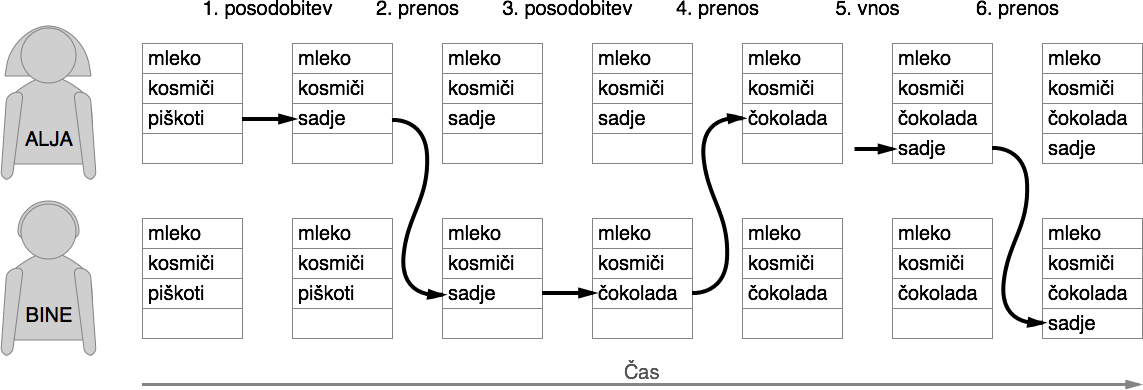
\includegraphics[width=16cm]{problem1.png}
\end{center}
\caption{Diagram sočasnega urejanja nakupovalnega listka, pri čemer mora Alja dvakrat vpisati svojo željo po sadju.}
\label{problem1}
\end{figure}

Pri tako fleksibilni interakciji lahko nastane konflikt. Alja bi lahko spremenila piškote v sadje sočasno kot bi Bine spremenil piškote v čokolado. Oba bi svoje spremembe videla takoj. Vendar spremembe Alje potrebujejo nekaj časa, da pridejo do Bineta. Tudi spremembe Bineta potrebujejo nekaj časa, da pridejo do Alje. Ta zamuda lahko spremeni vrstni red Aljine in Binetove spremembe, kar povzroči nakonsistentnost kot je to prikazano na Sliki \ref{problem2}. Alja in Bine bi morala pri sebi imeti vedno enake artikle na nakupovalnem listku.

\begin{figure}[placement h]
\begin{center}
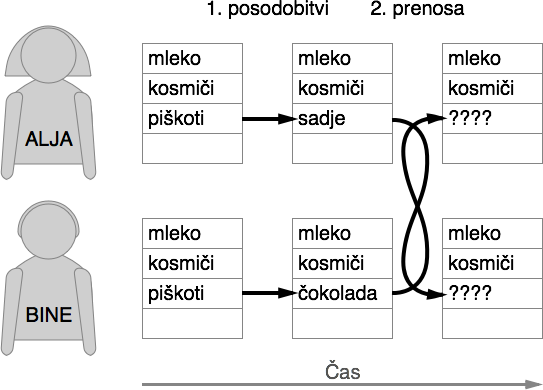
\includegraphics[width=8cm]{problem2.png}
\end{center}
\caption{Diagram sočasnega urejanja nakupovalnega listka. Vprašaji v zadnjem koraku pomenijo, da je seznam v konfliktu in mora biti razrešen, da zagotovimo konsistentnost. }
\label{problem2}
\end{figure}

\pagebreak

Predstavljajmo si enostavno rešitev za posodabljanja nakupovalnega listka, ki Alji in Binetu pokaže vedno zadnjo spremembo, ki je bila narejena na seznamu. Alja bi piškote spremenila v sadje, nato pa bi prišla Binetova sprememba v čokolado. Na drugi strani je Bine piškote spremenil v čokolado, nato pa bi sprejel Aljino sadje. V tem primeru bi Alja in Bine na koncu imela dva različna seznama, česar sploh ne bi opazila. Primer slabega reševanja konfliktov je prikazan na Sliki \ref{problem3}.

\begin{figure}[placement h]
\begin{center}
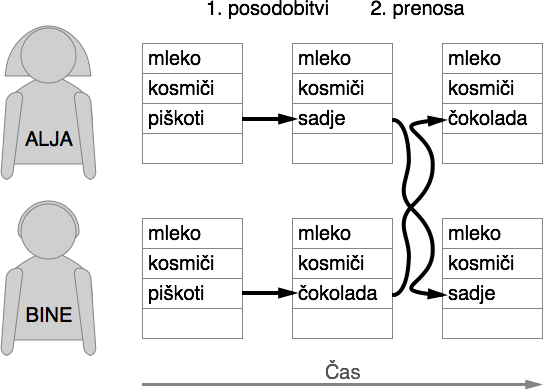
\includegraphics[width=8cm]{problem3.png}
\end{center}
\caption{Diagram sočasnega urejanja nakupovalnega listka. Konflikt v zadnjem koraku je rešen na način, da Alja in Bine sprejmeta zadnjo narejeno spremembo. Rešitev je slaba, saj ne zagotavlja konsistentnosti. }
\label{problem3}
\end{figure}

Problem nastane še večji pri sodelovanju večih uporabnikov in še z večjo zamudo pri dostavi sprememb na nakupovlnam listku. Recimo, da se Alji in Binetu pridruži še Cene. Bine ima počasen internet. Alja in Cene na seznam dodata in odstranita deset novih artiklov še preden Bine dobi eno spremembo. Medtem ko Bine ureja svoj seznam, so spremembe Alje in Ceneta še na poti k njemu. Za zagotovitev konsistentnosti bi morala aplikacija upoštevati zakasnjene oddaljene spremembe na osnovi prvotne verzije nakupovalnega listka.

%%%%%%%%%%%%%%%%%%%%%%%%%%%%%%%%%%%%%%%%%%%%%%%%%%%%%%%%%%%%%%%%%%%%%%%%%%%%%%%%%%%%%%%%%%%%%%%%%%%%%%%%%%%%%%%%%%
\chapter{Sodelovanje v realnem času}

Kako reševati konflikte in zagotoviti konsistentnost med oddaljenimi uporabniki pri sočasnem urejanju, je eden izmed glavnih izivov moje diplomske naloge. V tem poglavju bomo raziskali protokole, ki omogočajo sodelovanje uporabnikov v realnem času in teoretično rešujejo omenjena problema. Najbolj razširjeni so Operativna transformacija (ang. Operational transformation), Diferenčna sinhronizacija (ang. Differential synchronization) in protokol Brez operativne transformacije (ang. Without operational transformation, bolj znan pod kratico WOOT).

%%%%%%%%%%%%%%%%%%%%%%%%%%%%%%%%%%%%%%%%%%%%%%%%%%%%%%%%%%%%%%%%%%%%%%%%%%%%%%%%%%%%%%%%%%%%%%%%%%%%%%%%%%%%%%%%%%
\section{Operativna transformacija}

Operativna transformacija se je prvič omenjala v članku Concurrency Control in Groupware Systems. Pri Googlu so Operativno transformacijo vzeli za osnovno pri načrtovanju protokola Wave, kar nakazuje na njeno uporabnost.

Zaradi razumljivosti bomo besedilo, ki ga urejajo uporabniki, poimenovali dokument. Dokument je shranjen kot serija kronoloških sprememb narejenih na dokumentu. Primer spremembe je {\tt \{ Vstavi ‘M’ @11 \}}, ki pomeni “v dokumentu na lokacijo 11 vstavi črko M” ali {\tt \{ Pobriši @3-7 \}}, ki pomeni “v dokumentu pobriši vse znake med lokacijo 3 in 7”. Obstajajo še druge vrste sprememb kot so oblikovanja besedila, zaklep odstavka, razveljevitev spremembe... Zaradi enostavnosti razlage se bomo osredotočili le na omenjena dva tipa sprememb. Ko uporabnik ureja besedilo, ne spreminja osnovnih znakov, ki bi skupaj predstavljali besedilo kot dokument. Namesto tega se njegove spremembe shranjujejo v revizijski dnevnik. Seveda dokumenta kot zaključene celote znakov obstaja. Vendar pomembne so spremembe, ki so bile narejene na tem dokumentu. Če se urejanju skupnega dokumenta pridruži nov uporabnik, mu iz revizijskega dnevnika ponovimo vse (od prve do zadnje) spremembe in že lahko sodeluje pri urejanju tako kot ostali uporabniki.

Glede na to, da poznamo revizijo vseh sprememb narejenih na dokumentu, lahko preverimo, kaj je uporabnik imel v svojem urejevalniku, preden je naredil novo spremembo. Na ta način njegovo spremembo pravilno umestimo v skupno besedilo skupaj z ostalimi spremembami, ki so bile narejene med tem. Algoritem, ki skrbi za umeščanje ali združevanje (ang. merging) sprememb, se imenuje Operativna transformacija (v nadaljevanju OT).

\bigskip

Poglejmo delovanje OT na primeru. Predpostavimo, da imamo dokument v katerem se trenutno nahaja stavek “ENOSTAVNO KOT PASULJ” in zasede dvajset lokacij. Urejanju tega dokumenta se pridružita Alja in Bine. Če Bine spremeni stavek v “ENOSTAVNO KOT KEKS”, potem je za to moral narediti pet sprememb.

\begin{figure}[placement h]
\begin{center}
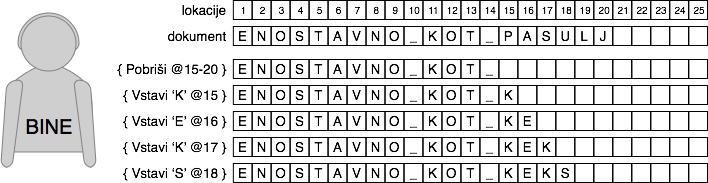
\includegraphics[width=12cm]{ot1.png}
\end{center}
\caption{Bine naredi pet sprememb.}
\label{ot1}
\end{figure}

Predstavljajmo si, da med tem ko Bine tipka, začne stavek spreminjati tudi Alja. in sicer v “TAKO ENOSTAVNO KOT PASULJ”. Tudi Alja je morala narediti pet sprememb.

\begin{figure}[placement h]
\begin{center}
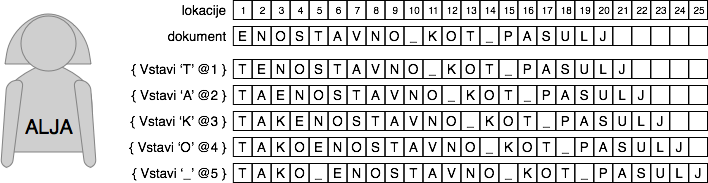
\includegraphics[width=12cm]{ot2.png}
\end{center}
\caption{Alja naredi pet sprememb.}
\label{ot2}
\end{figure}

Če bi Alja v naslednjem koraku naivno sprejela in izvršila Binetovo prvo spremembo, bi v stavku pobrisala napačne črke tako kot je to prikazano na Sliki \ref{ot3}.

\begin{figure}[placement h]
\begin{center}
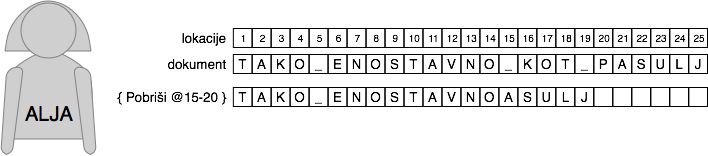
\includegraphics[width=12cm]{ot3.png}
\end{center}
\caption{Brez transformacije pride do nekonsistentnosti.}
\label{ot3}
\end{figure}

\pagebreak

Alja je imela pet znakov v začetku stavka, o katerih Bine še ni bil seznanjen. Lokacija Binetove spremembe je zato napačna glede na Aljino vezijo dokumenta. Da bi se izognili temu problemu, mora Alja narediti transformacijo Binetovih sprememb relativno na svoj lokalni dokument. V našem primeru, ko Alja sprejme Binetove spremembe, mora lokacijo spremembe zamakniti za pet znakov, kolikor jih je vpisala na začetku stavka. Ko naredi to transformacijo in izvrši Binetovo prvo spremembo, dobi pravilen stavek.

\begin{figure}[placement h]
\begin{center}
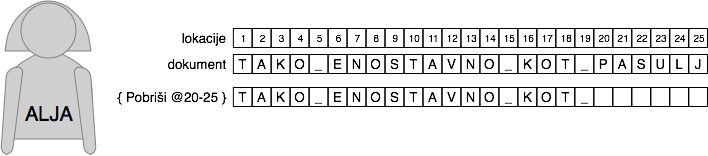
\includegraphics[width=12cm]{ot4.png}
\end{center}
\caption{Z uporabo Operativne transformacije dobimo pravilen rezultat.}
\label{ot4}
\end{figure}

Ko transformira in izvede še ostale štiri spremembe, dobi končno verzijo dokumenta.

\begin{figure}[placement h]
\begin{center}
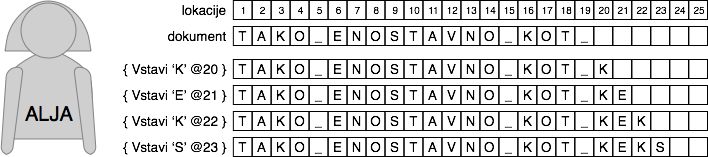
\includegraphics[width=12cm]{ot5.png}
\end{center}
\caption{Končna verzija dokumenta, ki ga vidi Alja.}
\label{ot5}
\end{figure}

Včasih spremembe ne povzročajo konfliktov in ni potrebe po transformaciji. Ko Bine prejme Aljine spremembe, ni potrebe po zamikanju lokacij. Bine mora izvesti Aljine spremembe točno take, kot jih je ona izvedla na svojem lokalnem dokumentu.

\begin{figure}[placement h]
\begin{center}
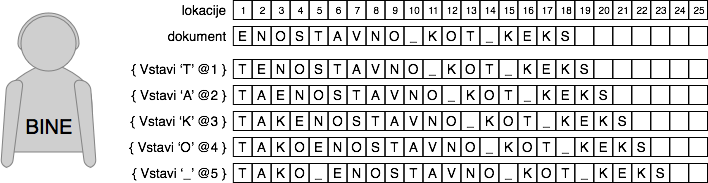
\includegraphics[width=12cm]{ot6.png}
\end{center}
\caption{Končna verzija dokumenta, ki ga vidi Bine.}
\label{ot6}
\end{figure}

Tako Alja kot Bine v svojem lokalnem dokumentu na koncu vidita stavek “TAKO ENOSTAVNO KOT KEKS”. Algoritem, ki smo ga uporabili za zamikanje sprememb, se imenuje Operativna transformacija. Pravilno implementiran algoritem nam garantira, da imajo vsi uporabniki, ko prejmejo vse spremembe, isto verzijo dokumenta.

%%%%%%%%%%%%%%%%%%%%%%%%%%%%%%%%%%%%%%%%%%%%%%%%%%%%%%%%%%%%%%%%%%%%%%%%%%%%%%%%%%%%%%%%%%%%%%%%%%%%%%%%%%%%%%%%%%
\subsection{Protokol sodelovanja}

Z OT smo se naučili, kako večim uporabnikom dopustiti urejanje istega dokument brez konflikov. Še vedno pa obstaja težava, kako vsako spremembo pravilno združiti z drugimi spremembami, če se le te zgodijo istočano. Zagotoviti moramo, da vsak oddaljeni uporabnik ve, da obstajajo spremembe, ki morajo biti združene. Za to skrbi Protokol sodelovanja (ang. Collaboartion protocol). Tehnologiji OT in Protokol sodelovanja skupaj, znak za znakom, skrbita za sodelovanja v realnem času.

Zavedati se moramo, da za urejanje dokumenta skrbijo tako strežnik kot odjemalec (običajno brskalniki uporabnikov). Pri urejanjeju dokumenta mora odjemalec sprocesirati vse sprembe, ki jih naredi uporabnik, in jih poslati na strežnik. Sprocesirati mora tudi vse spremebe drugih uporabnikov, ki mu jih pošlje strežnik.

Vsak odjemalec si mora beležiti:
\begin{list_type}
	\item Številko zadnje sinhornizirane revizije iz strežnika.
	\item Vse spremembe, ki so bile narejene lokalno in niso še bile poslane na strežnik.
	\item Vse spremembe, ki so bile narejene lokalno, poslane na strežnik, vendar jih strežnik še ni potrdil.
	\item Trenutno stanje dokumenta kot ga vidi sam uporabnik.
\end{list_type}

Na strežniku se shranjujejo tri stvari:
\begin{list_type}
	\item Seznam sprememb, ki jih je sprejel, a še ni sprocesiral.
	\item Revizijski dnevnik v katerem je celotna zgodovina sprememb.
	\item Trenutno stanje dokumenta.
\end{list_type}

S hranjenjem in uporabo teh informacij je mogoče zasnovati komunikacijo med strežnikom in odjemalci tako, da so oddaljeni urejevalniki drug od drugega sposobni naglo sprocesirati spremembe. Oglejmo si kako je v vzorčnem dokumentu poskrbljeno za komunikacijo med strežnikom in odjemalcem.

Na Sliki \ref{collab1} zunanja stolpce predstavljata uporabnika Aljo in Bineta, ki urejata skupni dokument. Srednji stolpec je strežnik. Spremembe, ki jih naredita Alja in Bine in se pošljejo na strežnik, so označene v ovalni obliki. Transformacije bodo na naslednjih slikah označene s kara obliko.

Recimo, da Alja začne tipkati “Pozdravljen” na začetku dokumenta.

\begin{figure}[placement h]
\begin{center}
\includegraphics[width=12cm]{collab1.png}
\end{center}
\caption{Alja začne tipkati “Pozdravljen”.}
\label{collab1}
\end{figure}

Aljin urejevalnik si spremembo shrani med “čekajoče spremembe”. V naslednjem trenutku se sprememba pošlje na server ter jo prastavi na seznam “poslanih sprememb”.

Alja nadaljuje s tipkanjem in doda “ svet” v svoj urejevalnik. V istem času Bine vpiše znak “!” v svoj prazen dokument. Bine še vedno ni prejel Aljinih sprememb.

\begin{figure}[placement h]
\begin{center}
\includegraphics[width=12cm]{collab2.png}
\end{center}
\caption{Alja nadaljuje s tipkanjem “ svet”. Bine na drugi strani vpiše “!”.}
\label{collab2}
\end{figure}

Aljin {\tt \{ Vstavi ‘svet’ @12 \}} je bil dodan med čakajoče spremembe in še ni poslan na strežnik. Pravilo je, da nikoli na server ne pošiljamo več kot ene čakajoče spremembe na enkrat. Dokler Alja od strežnika ne dobi potrditve prve spremembe, bo njen urejevalnik vse nove spremembe hranil med čakajočimi spremembami. Na Sliki \ref{collab3} lahko opazimo, da si je server Aljino prvo spremembo že shranil v revizijski dnevnik. V naslednjem koraku bo strežnik Binetu poslal Aljino prvo spremembo ter Alji odgovoril s potrditvijo, da si je zabeležil njeno spremembo.

\begin{figure}[placement h]
\begin{center}
\includegraphics[width=12cm]{collab3.png}
\end{center}
\caption{Strežnik procesira Aljino prvo spremembo.}
\label{collab3}
\end{figure}

Bine sprejme Aljino spremembo od strežnika, jo sprocesira v dokument ter posodobi številko zadnje sinhronizirane revizije na 1. Z uporabo OT mora transformirti svojo čakajoče spremembo {\tt \{ Vstavi ! @1 \}}. Ker je Alja na začetek dokumenta že vpisala “Pozdravljen”, Binetov urejevalnik njegovo spremembo zamakne za 11 mest. Alja je med tem sprejel potrditev iz strežnika. Tudi ona posodobi številko zadnje sinhronizirane revizije na 1, ter svojo spremembo odstrani iz seznama “poslanih sprememb”.

V naslednjem koraku bosta oba svoje “čakajoče spremembe” poslala na server, tako kot je to prikazano na Sliki \ref{collab4}.

\begin{figure}[placement h]
\begin{center}
\includegraphics[width=12cm]{collab4.png}
\end{center}
\caption{Sodelovanje Aljinega in Binetovega urejevalnika preko centralnega strežnika.}
\label{collab4}
\end{figure}



%%%%%%%%%%%%%%%%%%%%%%%%%%%%%%%%%%%%%%%%%%%%%%%%%%%%%%%%%%%%%%%%%%%%%%%%%%%%%%%%%%%%%%%%%%%%%%%%%%%%%%%%%%%%%%%%%%
\section{Diferenčna sinhronizacija}

Vestibulum leo elit, rutrum et ultricies at, tempus ut nibh. Donec tincidunt libero id congue tristique. Nulla in tortor magna. Donec quis dui elit. Suspendisse porttitor eros in eros malesuada, id fermentum est porta. Quisque in egestas mi. Vestibulum sodales magna erat, quis pretium metus luctus id. In ac justo ac arcu fermentum fringilla sit amet eu nibh. Nulla tempus iaculis venenatis. Curabitur id risus magna. Vestibulum in erat orci. Cras porttitor vitae tortor et feugiat. Praesent vitae facilisis nibh. Sed vel sodales ante. Proin sollicitudin massa eget ornare aliquet. Aliquam erat volutpat. Curabitur arcu arcu, egestas vitae orci et, condimentum ultricies leo. Suspendisse non leo nec eros pulvinar dignissim non vitae urna. Nulla lacinia facilisis consectetur. Fusce quis quam mollis, pharetra lacus in, pulvinar nisl. In vitae turpis risus. Vestibulum dapibus elementum malesuada. Morbi eleifend felis in nisi imperdiet, a iaculis enim sollicitudin. Integer fringilla purus nisi, dictum posuere nisi suscipit eget. In porttitor porta eros vitae hendrerit. Maecenas in varius lacus. Pellentesque eu congue nisl, id iaculis dolor. Maecenas a lacus a leo commodo egestas. Curabitur nec mi quam. Vestibulum elementum faucibus semper. Praesent quis urna sit amet arcu tempus facilisis non id est. Donec vestibulum dui a convallis lobortis. Pellentesque habitant morbi tristique senectus et netus et malesuada fames ac turpis egestas. Vivamus sodales tortor vitae dictum congue. Fusce lectus metus, auctor at ante sit amet, consequat tempus enim. Donec eget nisl commodo sapien accumsan aliquet volutpat eget ligula. Cras at auctor dui. Morbi odio tortor, mollis at orci non, elementum dictum ligula. Integer vehicula orci sit amet magna pharetra feugiat. Nam porta volutpat arcu, eu convallis dolor malesuada in. Donec iaculis commodo lorem eu aliquet. Ut vitae nulla aliquet dui molestie adipiscing dignissim et ipsum.

%%%%%%%%%%%%%%%%%%%%%%%%%%%%%%%%%%%%%%%%%%%%%%%%%%%%%%%%%%%%%%%%%%%%%%%%%%%%%%%%%%%%%%%%%%%%%%%%%%%%%%%%%%%%%%%%%%
\section{WOOT}

Pellentesque tempus felis eget ipsum commodo elementum. Integer quis lorem interdum, elementum dolor a, ornare erat. Praesent quis mauris sed justo aliquam pretium vel eget quam. Suspendisse potenti. Vestibulum venenatis, odio ac iaculis mattis, dui diam viverra libero, quis sollicitudin libero nisi id magna. Donec luctus feugiat bibendum. Ut nec vulputate risus. Nunc sit amet lobortis quam, sit amet malesuada leo. Proin erat nisi, rutrum sit amet est non, viverra mattis metus. Morbi scelerisque enim et eleifend bibendum. Etiam luctus risus vitae urna malesuada, vestibulum aliquet ipsum luctus. Donec nec velit porta, molestie libero quis, egestas lorem. Curabitur a mauris vitae velit tristique consequat ut non magna. Duis dictum ipsum vitae commodo tristique. Vestibulum posuere egestas leo, quis accumsan nulla dapibus eu. Morbi mi quam, consequat id fringilla quis, accumsan non nisi. Proin in lacinia purus. Sed et viverra eros. Nulla mollis lobortis lacus id aliquam. Donec ac aliquet purus, non vehicula augue. Cras at imperdiet metus. Nullam dignissim, mi eu eleifend luctus, neque enim volutpat neque, at sagittis neque mi eu nisl. Ut diam massa, feugiat sit amet malesuada vitae, porta eu eros. Suspendisse sit amet tincidunt mauris. Vestibulum accumsan ante quis mi sollicitudin pharetra a nec enim. Phasellus porta id risus ac consectetur. Donec aliquam tellus ut ante scelerisque, eget vehicula sem pellentesque. Aliquam erat volutpat. Praesent ut adipiscing nibh, at pellentesque eros. Integer pellentesque erat id accumsan lacinia. Vivamus neque nunc, condimentum lobortis adipiscing ac, volutpat quis lorem. Proin et neque sollicitudin, gravida quam lacinia, tristique mauris. Mauris at viverra massa. Nullam condimentum, arcu sit amet varius rutrum, leo libero mollis orci, quis aliquet nibh mauris quis tortor. Nulla vel lorem velit. Nullam tempus turpis eget porttitor auctor. Praesent sed fringilla dui. Vestibulum a magna id nunc interdum feugiat. Sed auctor vitae tortor id vehicula.

%%%%%%%%%%%%%%%%%%%%%%%%%%%%%%%%%%%%%%%%%%%%%%%%%%%%%%%%%%%%%%%%%%%%%%%%%%%%%%%%%%%%%%%%%%%%%%%%%%%%%%%%%%%%%%%%%%
\chapter{Modeli konsistence, struktura in pravilnost}

Nulla vel lorem erat. Nullam convallis molestie mauris non vulputate. Fusce sagittis purus non mi interdum, ac tempor nunc vulputate. Vivamus tempor diam a laoreet porta. Aliquam adipiscing elit vel risus accumsan, eget lacinia felis rutrum. Mauris ornare mattis vestibulum. Proin adipiscing semper turpis, eleifend sollicitudin tortor aliquam eget.

Nam non odio at arcu tincidunt laoreet. Aenean iaculis magna nec risus semper, eu hendrerit nunc blandit. Vivamus in eros sit amet augue interdum fringilla. Nullam semper volutpat iaculis. Aliquam erat volutpat. Nullam magna magna, adipiscing non leo imperdiet, pharetra facilisis ante. Mauris quis felis sed turpis sagittis varius. Quisque laoreet elementum mauris, ac lacinia magna ultricies ac. Praesent a blandit nibh. Maecenas malesuada velit ac accumsan convallis. Quisque ultrices arcu lacus, vulputate cursus arcu faucibus id. Suspendisse blandit at enim eu condimentum. Praesent laoreet luctus enim, nec ultrices est varius eu. Vestibulum viverra ante eu est ultrices feugiat eget nec mauris. Vestibulum tempus nisl risus, non condimentum ipsum elementum a. Maecenas ligula enim, consectetur sit amet dignissim eu, blandit nec enim. In hac habitasse platea dictumst. Praesent auctor ligula ut justo congue mattis. In mollis porta tempor. Cras tincidunt egestas porta. Donec non tristique arcu. Vestibulum tempor ac nisl non tincidunt. Duis hendrerit risus mi, ut commodo orci eleifend a. Aenean hendrerit leo sed consectetur facilisis. Duis gravida blandit accumsan. Curabitur id volutpat lorem. Nunc ac vulputate massa. Morbi aliquam cursus ligula id malesuada. Nam ut felis orci. Vestibulum tincidunt cursus mi, hendrerit scelerisque orci aliquet sit amet. Quisque placerat nunc sit amet nibh congue tincidunt. Sed vitae hendrerit mauris, in egestas leo. Etiam blandit hendrerit felis a malesuada. Cras ultricies urna sed tincidunt blandit. Donec at gravida purus, eu gravida augue. Curabitur varius nibh nec erat hendrerit blandit. Etiam commodo elit ut luctus elementum.

%%%%%%%%%%%%%%%%%%%%%%%%%%%%%%%%%%%%%%%%%%%%%%%%%%%%%%%%%%%%%%%%%%%%%%%%%%%%%%%%%%%%%%%%%%%%%%%%%%%%%%%%%%%%%%%%%%
%\section{Model CC}

In hac habitasse platea dictumst. Vestibulum lorem orci, suscipit eget fermentum nec, convallis in odio. Curabitur eu rhoncus eros, faucibus ullamcorper mi. Nam varius sapien tellus, et mollis nisl hendrerit venenatis. Vivamus facilisis lectus ac nisl porttitor, a placerat sem egestas. Aliquam ornare iaculis justo pellentesque venenatis. Donec euismod libero sed neque venenatis ullamcorper. Donec vestibulum quam lorem, id ornare sem sodales nec. Curabitur tristique nibh pellentesque, blandit leo at, hendrerit felis. Donec rhoncus massa non tortor condimentum semper. Nulla varius nulla vel elit vestibulum, nec malesuada nibh posuere. Vestibulum sagittis est nec laoreet lobortis. Proin eget varius quam. Vestibulum sit amet sodales libero, non commodo purus. Sed ullamcorper nulla a imperdiet dignissim. Aliquam sed turpis porta, rutrum erat nec, iaculis purus. Mauris gravida erat non tortor faucibus, vitae malesuada dolor vehicula. Morbi volutpat ipsum non mauris gravida luctus. Nunc venenatis molestie ligula, volutpat bibendum felis scelerisque eget. Phasellus eget lectus vitae nisi bibendum dignissim sit amet eget odio. Fusce sed ipsum in turpis feugiat dictum. Donec sed arcu orci. Nullam ac suscipit urna. Ut sollicitudin sagittis justo id volutpat.

%%%%%%%%%%%%%%%%%%%%%%%%%%%%%%%%%%%%%%%%%%%%%%%%%%%%%%%%%%%%%%%%%%%%%%%%%%%%%%%%%%%%%%%%%%%%%%%%%%%%%%%%%%%%%%%%%%
%\section{Model CSM}

Etiam blandit diam in tincidunt facilisis. Donec mi est, malesuada et felis non, condimentum cursus nisl. Sed sit amet nisi ac massa eleifend commodo ut a enim. Fusce congue at dui at aliquet. Sed et nisi facilisis, dapibus elit nec, lobortis libero. Sed a orci et ante venenatis feugiat. Praesent quis sodales mauris, id tincidunt eros. Suspendisse potenti. Vestibulum leo neque, vulputate mattis mollis ac, ultricies eget mi. Proin tortor ligula, fringilla nec sapien et, rhoncus rutrum augue. Vestibulum ut tellus laoreet, congue elit eget, semper sapien. Cras diam mi, lobortis ut vehicula ut, hendrerit vel nisi. Quisque auctor dui id enim iaculis, ac varius nisl porttitor. Cras in lectus vulputate, rutrum risus ut, ornare nisl. Sed viverra ligula vel tristique sagittis. Donec non leo eu lorem ultricies congue nec nec lacus. Maecenas egestas sed augue nec sodales. Integer ac leo eu risus pharetra auctor vitae non nibh. Cras in purus eu eros imperdiet mattis in sed ligula. Pellentesque id varius sem. Ut et velit mattis lacus sagittis egestas non ac lectus. Proin eget neque mi. Maecenas molestie, sapien vitae tincidunt luctus, felis sapien semper diam, ac consectetur augue lacus vitae augue. Vivamus bibendum libero eu elit lobortis elementum. Integer mollis neque et sapien vestibulum cursus. In eget elit eu ligula aliquam sollicitudin. Curabitur iaculis vel lorem id fermentum. Curabitur ante massa, laoreet in semper eget, interdum ac magna. Vestibulum tincidunt dignissim volutpat. Phasellus urna velit, imperdiet quis semper quis, rhoncus nec est. Aliquam mauris nunc, tincidunt a placerat vitae, scelerisque quis lorem.

%%%%%%%%%%%%%%%%%%%%%%%%%%%%%%%%%%%%%%%%%%%%%%%%%%%%%%%%%%%%%%%%%%%%%%%%%%%%%%%%%%%%%%%%%%%%%%%%%%%%%%%%%%%%%%%%%%
%\section{Model CA}

Interdum et malesuada fames ac ante ipsum primis in faucibus. Nam sagittis ipsum nisi, at ultricies nisl interdum sed. Nulla facilisi. Vestibulum tristique nunc ipsum, nec luctus tellus vulputate sit amet. Sed diam justo, imperdiet eu magna ut, convallis accumsan neque. Nulla non dolor volutpat, mollis justo vitae, auctor est. Nunc id mi nulla. Integer aliquet, tellus id dictum lobortis, arcu urna posuere lectus, in rutrum orci sapien in ante. Etiam aliquam turpis sapien, quis varius nisl pretium accumsan. Suspendisse ultrices nibh sed libero fermentum, et scelerisque turpis pretium. Sed lobortis nibh eu ante scelerisque auctor. Donec eu interdum metus, et dignissim nulla. Maecenas vestibulum rutrum lacus. Fusce fringilla metus hendrerit, ultricies velit at, blandit libero. Nulla nisl eros, adipiscing in mauris eu, ullamcorper pretium augue. Ut imperdiet odio vitae velit imperdiet, id consectetur lorem rutrum. Interdum et malesuada fames ac ante ipsum primis in faucibus. Quisque risus sapien, molestie ut tortor sed, sollicitudin pulvinar magna. Donec a quam quam. Proin hendrerit purus in sapien consequat tristique. Donec malesuada quis odio non varius. Mauris lobortis, eros eget euismod commodo, magna odio eleifend mi, sed ullamcorper leo massa vitae sem. Nullam eros enim, luctus nec ante quis, varius molestie lorem. Praesent ullamcorper, ante ac faucibus adipiscing, urna urna porttitor arcu, at luctus velit erat vitae elit. Fusce dui quam, vulputate vel cursus non, pulvinar sed ante. Nullam interdum turpis in libero tempor, non sodales leo consectetur. Donec quis eros non quam fermentum varius et ut neque. Nulla vel dolor velit. Aliquam erat volutpat. Sed fringilla quam a sem fringilla lacinia. In condimentum ante nisl, eget egestas urna pretium vitae. Vivamus facilisis feugiat mi, sit amet congue dui aliquam id. Maecenas luctus sed lorem vitae auctor. Maecenas eu magna sed nisl lobortis commodo.

Sed condimentum nisi augue, vitae scelerisque dui congue at. Pellentesque ac sem sed velit faucibus rutrum. Proin fringilla nunc eu dui rutrum, vel luctus nunc dapibus. Nullam mi enim, convallis ac sapien et, suscipit pellentesque lorem. Duis ornare massa nec quam gravida laoreet. Nam ut semper sapien. Aenean quis massa nisi. Praesent quis ligula vel dolor ornare interdum tempus quis urna. Mauris quis justo id lorem porttitor egestas eget ornare arcu. Vestibulum et turpis arcu. Vivamus et placerat mauris. Proin eget eleifend diam, sit amet pharetra leo. Proin auctor vulputate nisl, at placerat massa. Sed tempor mi at varius facilisis.

%%%%%%%%%%%%%%%%%%%%%%%%%%%%%%%%%%%%%%%%%%%%%%%%%%%%%%%%%%%%%%%%%%%%%%%%%%%%%%%%%%%%%%%%%%%%%%%%%%%%%%%%%%%%%%%%%%
\chapter{Algoritmi integracije operativne transformacije}

Phasellus felis diam, molestie in laoreet ac, vestibulum at nunc. Donec et venenatis leo. Nunc elementum molestie est in tincidunt. Integer suscipit, tortor a sodales fringilla, lacus turpis hendrerit elit, tempor pharetra metus sapien ac nisl. Nam vitae neque ipsum. Cras porttitor enim tortor, ut ultricies mi fermentum vitae. Sed at pretium diam. Phasellus eros felis, lacinia et pellentesque sed, feugiat ac ante. Donec sed imperdiet leo. Pellentesque eu luctus lacus. Integer adipiscing lectus a gravida scelerisque. Nam fermentum turpis et posuere semper. Maecenas sit amet sapien lorem. Aenean mattis auctor nibh, nec congue enim varius id. Quisque eget enim eu lectus accumsan vulputate vitae id urna. Donec non felis nec ipsum semper luctus vel eu nisi.

Cras dapibus lacus metus, id tristique odio feugiat sit amet. Etiam erat odio, ornare et eros semper, lacinia ornare metus. Sed vestibulum dolor id leo faucibus, a egestas massa tincidunt. Morbi libero quam, lacinia ac dapibus vel, scelerisque eu libero. Aenean suscipit purus vel diam congue, eget fringilla orci fringilla. Donec purus augue, varius nec tortor vel, lacinia pulvinar libero. Vestibulum at adipiscing lacus. Phasellus at vestibulum lectus.

%%%%%%%%%%%%%%%%%%%%%%%%%%%%%%%%%%%%%%%%%%%%%%%%%%%%%%%%%%%%%%%%%%%%%%%%%%%%%%%%%%%%%%%%%%%%%%%%%%%%%%%%%%%%%%%%%%
\section{Pristop GROVE (decentraliziran)}

Cras dictum laoreet mi at lacinia. Sed nec volutpat leo. Nulla facilisi. Sed at orci ante. Integer id dui lectus. Maecenas sagittis, libero molestie varius lobortis, urna sapien congue magna, non commodo est turpis quis lacus. Vestibulum molestie tristique auctor. Etiam eget interdum diam. Donec at velit adipiscing purus tincidunt placerat. Donec luctus nulla sit amet felis ullamcorper, vel suscipit velit hendrerit. Fusce tempus magna dictum, volutpat metus id, commodo nunc. Etiam eu velit sapien. Phasellus accumsan, nunc convallis suscipit viverra, diam leo sagittis dolor, ac porta nulla libero porta tellus. Donec volutpat, massa nec pulvinar consectetur, eros elit vehicula dui, ut vehicula libero leo ut massa. Sed eget tempor augue.

Nullam sollicitudin nisi sed lacus tempus vehicula. Ut posuere tortor sem, aliquet tempor libero vestibulum vel. Nunc luctus, nibh semper bibendum lacinia, neque nisl dapibus purus, id consectetur lorem arcu a mi. Aenean vulputate non mi non auctor. Integer ultricies arcu scelerisque risus pharetra auctor. Nulla vulputate blandit dui, id euismod eros blandit congue. Curabitur porttitor dolor justo, ac gravida est rutrum tristique. Praesent in mattis diam, at aliquet tellus. Vestibulum ante ipsum primis in faucibus orci luctus et ultrices posuere cubilia Curae; Integer commodo purus non est feugiat tincidunt. Integer nisi dolor, porta eget nisi non, blandit feugiat tellus. Nam ac orci sed sapien cursus aliquet vitae in diam. Aliquam pulvinar libero id nibh scelerisque condimentum nec non elit. Nam tristique dui quis enim pretium fringilla.

%%%%%%%%%%%%%%%%%%%%%%%%%%%%%%%%%%%%%%%%%%%%%%%%%%%%%%%%%%%%%%%%%%%%%%%%%%%%%%%%%%%%%%%%%%%%%%%%%%%%%%%%%%%%%%%%%%
\section{Pristop Jupiter (odjemalec-strežnik)}

Donec sed eros venenatis, facilisis quam non, aliquam libero. Vivamus in vulputate leo. Integer tellus ipsum, venenatis ut sagittis eu, elementum eu nisi. Curabitur sit amet consectetur sem. Nulla in velit sed arcu ultrices fermentum. Fusce in est at sem interdum sagittis vel ac tellus. Suspendisse eget facilisis eros. Nunc non massa nec nisl hendrerit vestibulum non nec leo. Duis sollicitudin dapibus ante eu euismod. Morbi egestas tempor cursus.

Class aptent taciti sociosqu ad litora torquent per conubia nostra, per inceptos himenaeos. Proin tempor, quam pulvinar sagittis scelerisque, libero erat hendrerit dolor, et lacinia ipsum justo sit amet leo. Vestibulum mauris lectus, vestibulum quis porttitor at, pretium et elit. In dictum purus erat, ut imperdiet velit blandit ut. Sed rutrum diam dictum magna blandit suscipit. Sed a ipsum sed risus gravida suscipit a at purus. Cras molestie enim sed auctor porta.

Donec malesuada, tellus quis gravida malesuada, est nisl dapibus odio, non molestie elit velit non mi. Nulla facilisi. Nullam ut diam ac mi vestibulum tristique eget luctus nisi. In euismod diam quis convallis bibendum. Donec laoreet sem ac lectus porttitor, eu porttitor augue euismod. Ut vulputate condimentum orci, ut tincidunt sem rhoncus eu. Nulla consequat porta ligula, nec lobortis lectus vehicula in. Aenean ac bibendum justo, lacinia pellentesque nulla. Etiam nec cursus ante.

%%%%%%%%%%%%%%%%%%%%%%%%%%%%%%%%%%%%%%%%%%%%%%%%%%%%%%%%%%%%%%%%%%%%%%%%%%%%%%%%%%%%%%%%%%%%%%%%%%%%%%%%%%%%%%%%%%
\section{Pristop Google Wave (izboljšava)	}

Maecenas consequat adipiscing ligula, a imperdiet ligula tincidunt ut. Sed a tristique quam. Sed quis posuere lorem. In suscipit lacus eu velit pellentesque scelerisque. Etiam pretium in mi vel placerat. Nunc at ultrices lacus, id tincidunt magna. Vivamus ac nibh ac quam vulputate luctus. Pellentesque id eros eu sem facilisis tincidunt. Donec varius odio ut elit porttitor, quis lobortis turpis porttitor. Nunc dui dolor, molestie ac odio quis, porta sollicitudin tellus. Donec commodo metus id sodales suscipit. Sed nec lectus adipiscing, feugiat ante id, sollicitudin neque. Aliquam blandit adipiscing neque, eget feugiat urna viverra sit amet.

Aenean porta, ligula ut feugiat porta, metus felis \cite{gdocs} fermentum sem, quis aliquam lectus erat nec lectus. Maecenas vitae est felis. Nunc sit amet pharetra mauris, semper fermentum lorem. Nam lobortis egestas blandit. Donec mattis quis metus sed accumsan. Pellentesque in pulvinar massa. Donec at nisi nec turpis porta molestie. Vestibulum gravida ac lacus sit amet dignissim. Proin risus ligula, rhoncus ac sapien non, dignissim convallis lorem. Suspendisse vehicula et dolor eu ultrices.

%%%%%%%%%%%%%%%%%%%%%%%%%%%%%%%%%%%%%%%%%%%%%%%%%%%%%%%%%%%%%%%%%%%%%%%%%%%%%%%%%%%%%%%%%%%%%%%%%%%%%%%%%%%%%%%%%%
\chapter{Urejevalniki v realnem času}

Quisque ut velit bibendum, convallis urna vitae, tempor felis. Fusce cursus condimentum nisl, accumsan pharetra lorem iaculis sit amet. In ac lectus est. Nulla facilisi. Vivamus ornare justo id neque interdum, auctor ornare turpis cursus. Vestibulum euismod nisl orci. Curabitur consectetur, nibh vel tristique pretium, enim magna hendrerit tortor, non rutrum risus nibh et urna. Vivamus a ornare libero. Integer vitae tortor tincidunt, placerat mauris ac, molestie risus. Pellentesque ipsum neque, molestie nec malesuada blandit, fringilla cursus sapien. Sed sed risus lacinia, tempus tortor at, cursus metus. In lacinia elit vel est varius, feugiat faucibus libero vulputate. Nam molestie enim ut interdum venenatis. Donec dolor arcu, blandit et tempor nec, cursus a leo. Phasellus id sollicitudin sapien. Aenean placerat adipiscing metus eget rutrum. Proin adipiscing ac dui vel rutrum. Aenean sit amet placerat nibh. Nulla tempus tristique tortor in auctor. Fusce volutpat mattis fermentum. Maecenas accumsan nibh ut nisi consequat, eget blandit augue auctor. Aenean ac elementum mi. Aenean eu mattis ipsum. Vivamus dolor ipsum, aliquet id dapibus mattis, pretium vel enim.

%%%%%%%%%%%%%%%%%%%%%%%%%%%%%%%%%%%%%%%%%%%%%%%%%%%%%%%%%%%%%%%%%%%%%%%%%%%%%%%%%%%%%%%%%%%%%%%%%%%%%%%%%%%%%%%%%%
\chapter{Poskus implementacije OT}

Sed nec luctus elit. Etiam feugiat, ipsum at fringilla iaculis, ligula massa auctor lorem, quis viverra ligula quam ut orci. Ut faucibus consectetur velit vel adipiscing. Aliquam nec metus sapien. Morbi nec lobortis ipsum. Etiam vehicula, libero dapibus pulvinar pretium, orci nunc aliquam leo, id bibendum lacus diam id quam. Etiam at lectus ac mi malesuada ultricies. Cras id venenatis nisl. Mauris ullamcorper felis eget arcu rhoncus ullamcorper. Nullam sollicitudin justo in orci iaculis, eget tristique tellus adipiscing. Sed at bibendum felis, viverra mollis est. Proin convallis felis eget augue condimentum, at placerat sem porttitor. Sed turpis nulla, fringilla sit amet ultrices id, condimentum ut massa. Pellentesque nec augue a mauris commodo suscipit et in ante. Praesent mollis et diam nec fermentum.

\begin{lstlisting}[caption={Interdum pretium}, label={lst:codeJavaScript}, title={Exampelus \ref{lst:codeJavaScript}: Interdum pretium}]
function cache_add () {
	var self = this;

	@\label{lst:codeJavaScript_mark}@self.cache.add(self.user._id + '_testing', self.resource('sl', 'session_dafaq'));

	self.json({
		status: 'okay',
		text: self.resource('sl', 'cache_has_been_successfully_set')
	}); return;
}
\end{lstlisting}

Pellentesque egestas orci quis dui tincidunt \ref{lst:codeJavaScript} io linus \ref{lst:codeJavaScript_mark} fringilla. Vivamus ac libero arcu. Mauris hendrerit massa eros. Morbi augue ligula, viverra sed volutpat at, pharetra ut erat. Integer consectetur tristique diam, vulputate placerat urna fermentum eu. Ut feugiat ligula a quam venenatis gravida. Ut elementum fermentum sapien, at posuere purus lacinia non. Mauris ante nunc, sodales eu pretium vitae, ultrices ac turpis.

%%%%%%%%%%%%%%%%%%%%%%%%%%%%%%%%%%%%%%%%%%%%%%%%%%%%%%%%%%%%%%%%%%%%%%%%%%%%%%%%%%%%%%%%%%%%%%%% sklpne ugotovitve
\chapter{Sklepne ugotovitve}

Nam semper augue at rhoncus laoreet. Nunc non aliquet risus. Curabitur dictum, nisl nec interdum pretium, dui quam vehicula urna, vel porta nunc est rutrum tellus. Aliquam condimentum pharetra sem, sed sodales massa viverra id. Nam aliquam faucibus egestas. Cras viverra non augue sed sagittis. Nam et elit a tortor aliquet laoreet. Pellentesque congue, risus ultricies rhoncus tincidunt, quam libero tempor tellus, sit amet bibendum velit augue eleifend lectus. Integer lorem nulla, placerat varius faucibus eu, cursus tempor purus. Cras at suscipit elit. Nam varius in ipsum eget tristique. Nulla ac nulla rutrum, vulputate lacus ac, dignissim ligula. Mauris imperdiet ut leo a tempus. Aliquam tempor condimentum massa, at varius diam egestas nec. Mauris eu sem at odio sagittis porta. Curabitur quis rhoncus magna, vitae dignissim enim.

%%%%%%%%%%%%%%%%%%%%%%%%%%%%%%%%%%%%%%%%%%%%%%%%%%%%%%%%%%%%%%%%%%%%%%%%%%%%%%%%%%%%%%%%%%%%%%%%%%%%%%% literatura
\addcontentsline{toc}{chapter}{Literatura}
\begin{thebibliography}{99}
\bibitem{problem} The Dojo Fundation. Open Cooperative Web Framework. Dostopno na:\\ http://opencoweb.org/ocwdocs/intro/openg.html
\bibitem{gdocs} J. Day-Richter. What’s different about the new Google Docs. Dostopno na:\\ http://googledocs.blogspot.com/2010/09/whats-different-about-new-google-docs\_22.html
\bibitem{diffsync} Neil Fraser. Differential Synchronization. Dostopno na:\\ https://neil.fraser.name/writing/sync/
\bibitem{woot} G. Oster, P. Urso, P. Molli, A. Imine. Real time group editors without Operational transformation. Dostopno na:\\ http://hal.inria.fr/docs/00/07/12/40/PDF/RR-5580.pdf
\bibitem{faq} C. Sun. Operational Transformation Frequently Asked Questions and Answers. Dostopno na:\\ http://cooffice.ntu.edu.sg/otfaq/
\bibitem{grove} C.A. Ellis, S.J. Gibbs. “Concurrency Control in Groupware Systems”. Dostopna na:\\ http://www-ihm.lri.fr/~mbl/ENS/CSCW/2012/papers/Ellis-SIGMOD89.pdf
\bibitem{jupiter} D. A. Nichols, P. Curtis, M. Dixon, J. Lamping. “High-Latency, Low-Bandwidth Windowing in the Jupiter Collaboration System”. Dostopno na:\\ http://lively-kernel.org/repository/webwerkstatt/!svn/bc/15693/projects/Collaboration/paper/Jupiter.pdf
\bibitem{wave} D. Wang, A. Mah, S. Lassen. Google Wave Operational Transformation. Dostopno na:\\ http://www.waveprotocol.org/whitepapers/operational-transform
\end{thebibliography}

%%%%%%%%%%%%%%%%%%%%%%%%%%%%%%%%%%%%%%%%%%%%%%%%%%%%%%%%%%%%%%%%%%%%%%%%%%%%%%%%%%%%%%%%%%%%%%%%%%%%%%%%%%%%%%%%%%
\end{document}